\documentclass[tikz,border=8pt]{standalone}
\usepackage{amsmath}
\usepackage{amssymb}
\usepackage{tikz}
\usetikzlibrary{arrows.meta,calc,decorations.pathreplacing,patterns,shapes.geometric,positioning,shadings,plotmarks}

\begin{document}
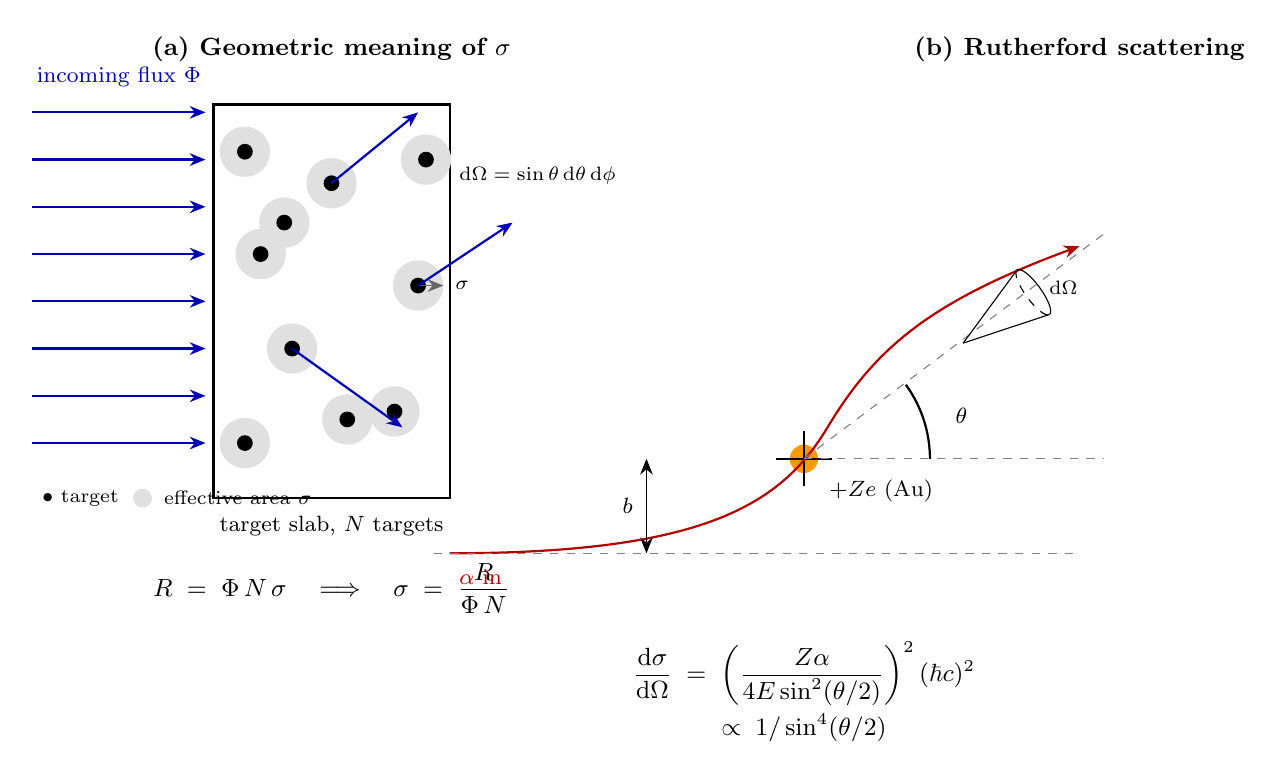
\begin{tikzpicture}[>={Stealth[length=2mm,width=1.6mm]}]

%================ LEFT PANEL: cross section geometric definition ================
\begin{scope}[shift={(0,0)}]

% Title
\node[font=\small\bfseries] at (3.5,5.2) {(a) Geometric meaning of $\sigma$};

% Target box
\draw[thick,black] (2.0,-0.5) rectangle (5.0,4.5);
\node[font=\footnotesize] at (3.5,-0.85) {target slab, $N$ targets};

% Effective area (light gray) plus solid black target dots
% Random-ish but non-overlapping placements
\foreach \x/\y in {2.4/0.2, 3.0/1.4, 4.3/0.6, 2.6/2.6, 4.6/2.2, 3.5/3.5, 4.7/3.8, 2.4/3.9, 3.7/0.5, 2.9/3.0}{
  \fill[black!12] (\x,\y) circle (0.32);
  \fill[black] (\x,\y) circle (0.10);
}

% Mark sigma on one target
\draw[->,thin,black!60] (4.6,2.2) -- ++(0.32,0.0);
\node[font=\scriptsize,anchor=west] at (4.95,2.2) {$\sigma$};

% Incoming flux (blue arrows from the left)
\foreach \y in {0.2,0.8,1.4,2.0,2.6,3.2,3.8,4.4}{
  \draw[->,thick,blue!70!black] (-0.3,\y) -- (1.9,\y);
}
\node[font=\footnotesize,blue!70!black] at (0.8,4.85) {incoming flux $\Phi$};

% Some scattered (deflected) outgoing arrows
\draw[->,thick,blue!70!black] (4.6,2.2) -- (5.8,3.0);
\draw[->,thick,blue!70!black] (3.5,3.5) -- (4.6,4.4);
\draw[->,thick,blue!70!black] (3.0,1.4) -- (4.4,0.4);

% Formula
\node[font=\small,anchor=north] at (3.5,-1.2) {$R \;=\; \Phi\, N\, \sigma \quad\Longrightarrow\quad \sigma \;=\; \dfrac{R}{\Phi\, N}$};

% Legend
\node[font=\scriptsize,anchor=west] at (-0.3,-0.5) {$\bullet$ target};
\fill[black!12] (1.1,-0.5) circle (0.12);
\node[font=\scriptsize,anchor=west] at (1.25,-0.5) {effective area $\sigma$};

\end{scope}

%================ RIGHT PANEL: Rutherford scattering geometry ================
\begin{scope}[shift={(9.5,0)}]

% Title
\node[font=\small\bfseries] at (3.5,5.2) {(b) Rutherford scattering};

% Target nucleus at origin (use a plus marker, gold tone)
\fill[orange!80!yellow] (0,0) circle (0.18);
\draw[thick,black] (-0.35,0) -- (0.35,0);
\draw[thick,black] (0,-0.35) -- (0,0.35);
\node[font=\footnotesize,anchor=north west] at (0.2,-0.15) {$+Ze$ (Au)};

% Hyperbolic trajectory: incoming from lower-left, scattered upward
% Use plot with a smooth path: parametric hyperbola
% Asymptotes: incoming along angle 0 (horizontal from left), outgoing along theta
% We approximate with a smooth bezier
\draw[thick,red!70!black,->] (-4.5,-1.2) .. controls (-1.3,-1.2) and (-0.3,-0.6) .. (0.3,0.4)
    .. controls (0.9,1.4) and (1.6,2.0) .. (3.5,2.7);

% Incoming straight asymptote (dashed) for reference and impact parameter
\draw[dashed,gray] (-4.7,-1.2) -- (3.5,-1.2);

% Impact parameter b (vertical between origin and incoming asymptote)
\draw[<->,thin,black] (-2.0,-1.2) -- (-2.0,0);
\node[font=\footnotesize,anchor=east] at (-2.05,-0.6) {$b$};

% Outgoing asymptote (dashed)
\draw[dashed,gray] (0,0) -- (3.8,2.85);

% Forward direction (dashed, continuing incoming)
\draw[dashed,gray] (0,0) -- (3.8,0);

% Scattering angle theta arc
\draw[thick,black] (1.6,0) arc (0:36:1.6);
\node[font=\footnotesize] at (2.0,0.55) {$\theta$};

% Solid angle cone d Omega along the outgoing direction
% Outgoing direction angle ~ 36 degrees
\begin{scope}[rotate around={36:(0,0)}]
  \draw[thin,black] (2.5,0) -- (3.6,0.35);
  \draw[thin,black] (2.5,0) -- (3.6,-0.35);
  \draw[thin,black] (3.6,0.35) arc (90:-90:0.10 and 0.35);
  \draw[thin,dashed,black] (3.6,0.35) arc (90:270:0.10 and 0.35);
  \node[font=\scriptsize,anchor=west] at (3.7,0) {$\mathrm{d}\Omega$};
\end{scope}

% Label incoming alpha
\node[font=\footnotesize,red!70!black,anchor=west] at (-4.5,-1.5) {$\alpha$ in};

% Formula
\node[font=\small,anchor=north,align=center] at (0.0,-2.2) {%
  $\dfrac{\mathrm{d}\sigma}{\mathrm{d}\Omega} \;=\; \left(\dfrac{Z\alpha}{4E\sin^{2}(\theta/2)}\right)^{2}(\hbar c)^{2}$ \\[2pt]
  $\propto\; 1/\sin^{4}(\theta/2)$};

% solid angle definition
\node[font=\scriptsize,anchor=west] at (-4.5,3.6) {$\mathrm{d}\Omega = \sin\theta\,\mathrm{d}\theta\,\mathrm{d}\phi$};

\end{scope}

\end{tikzpicture}
\end{document}
